%%%%%%%%%%%%%%%%%%%%%%%%%%%%%%%%%%%%%%%%%
%  My documentation report
%  Objetive: Explain what I did and how, so someone can continue with the investigation
%
% Important note:
% Chapter heading images should have a 2:1 width:height ratio,
% e.g. 920px width and 460px height.
%
%%%%%%%%%%%%%%%%%%%%%%%%%%%%%%%%%%%%%%%%%


%----------------------------------------------------------------------------------------
%	PACKAGES AND OTHER DOCUMENT CONFIGURATIONS
%----------------------------------------------------------------------------------------

\documentclass[11pt,fleqn]{book} % Default font size and left-justified equations

\usepackage[top=3cm,bottom=3cm,left=3.2cm,right=3.2cm,headsep=10pt,letterpaper]{geometry} % Page margins

\usepackage{xcolor} % Required for specifying colors by name
\definecolor{ocre}{RGB}{52,177,201} % Define the orange color used for highlighting throughout the book


% Font Settings
\usepackage{avant} % Use the Avantgarde font for headings
%\usepackage{times} % Use the Times font for headings
\usepackage{mathptmx} % Use the Adobe Times Roman as the default text font together with math symbols from the Sym­bol, Chancery and Com­puter Modern fonts
\usepackage{microtype} % Slightly tweak font spacing for aesthetics

\usepackage[utf8]{inputenc} % Required for including letters with accents
\usepackage{amsmath,amssymb}
\usepackage[russian]{babel}
\usepackage[T1]{fontenc} % Use 8-bit encoding that has 256 glyphs

 
\urlstyle{same}

% Bibliography
\usepackage[style=alphabetic,sorting=nyt,sortcites=true,autopunct=true,babel=hyphen,hyperref=true,abbreviate=false,backref=true,backend=biber]{biblatex}
\addbibresource{bibliography.bib} % BibTeX bibliography file
\defbibheading{bibempty}{}

%----------------------------------------------------------------------------------------
%	VARIOUS REQUIRED PACKAGES
%----------------------------------------------------------------------------------------

\usepackage{titlesec} % Allows customization of titles

\usepackage{graphicx} % Required for including pictures
\graphicspath{{pic/}} % Specifies the directory where pictures are stored
% \graphicspath{{Plots/}}
\usepackage{lipsum} % Inserts dummy text

\usepackage{hyperref}


\usepackage{tikz} % Required for drawing custom shapes


\usepackage{enumitem} % Customize lists
\setlist{nolistsep} % Reduce spacing between bullet points and numbered lists

\usepackage{booktabs} % Required for nicer horizontal rules in tables

\usepackage{eso-pic} % Required for specifying an image background in the title page

%----------------------------------------------------------------------------------------
%	MAIN TABLE OF CONTENTS
%----------------------------------------------------------------------------------------

\usepackage{titletoc} % Required for manipulating the table of contents

\contentsmargin{0cm} % Removes the default margin
% Chapter text styling
\titlecontents{chapter}[1.25cm] % Indentation
{\addvspace{15pt}\large\sffamily\bfseries} % Spacing and font options for chapters
{\color{ocre!60}\contentslabel[\Large\thecontentslabel]{1.25cm}\color{ocre}} % Chapter number
{}  
{\color{ocre!60}\normalsize\sffamily\bfseries\;\titlerule*[.5pc]{.}\;\thecontentspage} % Page number
% Section text styling
\titlecontents{section}[1.25cm] % Indentation
{\addvspace{5pt}\sffamily\bfseries} % Spacing and font options for sections
{\contentslabel[\thecontentslabel]{1.25cm}} % Section number
{}
{\sffamily\hfill\color{black}\thecontentspage} % Page number
[]
% Subsection text styling
\titlecontents{subsection}[1.25cm] % Indentation
{\addvspace{1pt}\sffamily\small} % Spacing and font options for subsections
{\contentslabel[\thecontentslabel]{1.25cm}} % Subsection number
{}
{\sffamily\;\titlerule*[.5pc]{.}\;\thecontentspage} % Page number
[] 

%----------------------------------------------------------------------------------------
%	MINI TABLE OF CONTENTS IN CHAPTER HEADS
%----------------------------------------------------------------------------------------

% Section text styling
\titlecontents{lsection}[0em] % Indendating
{\footnotesize\sffamily} % Font settings
{}
{}
{}

% Subsection text styling
\titlecontents{lsubsection}[.5em] % Indentation
{\normalfont\footnotesize\sffamily} % Font settings
{}
{}
{}
 
%----------------------------------------------------------------------------------------
%	PAGE HEADERS
%----------------------------------------------------------------------------------------

\usepackage{fancyhdr} % Required for header and footer configuration

\pagestyle{fancy}
\renewcommand{\chaptermark}[1]{\markboth{\sffamily\normalsize\bfseries\chaptername\ \thechapter.\ #1}{}} % Chapter text font settings
\renewcommand{\sectionmark}[1]{\markright{\sffamily\normalsize\thesection\hspace{5pt}#1}{}} % Section text font settings
\fancyhf{} \fancyhead[LE,RO]{\sffamily\normalsize\thepage} % Font setting for the page number in the header
\fancyhead[LO]{\rightmark} % Print the nearest section name on the left side of odd pages
\fancyhead[RE]{\leftmark} % Print the current chapter name on the right side of even pages
\renewcommand{\headrulewidth}{0.5pt} % Width of the rule under the header
\addtolength{\headheight}{2.5pt} % Increase the spacing around the header slightly
\renewcommand{\footrulewidth}{0pt} % Removes the rule in the footer
\fancypagestyle{plain}{\fancyhead{}\renewcommand{\headrulewidth}{0pt}} % Style for when a plain pagestyle is specified

% Removes the header from odd empty pages at the end of chapters
\makeatletter
\renewcommand{\cleardoublepage}{
\clearpage\ifodd\c@page\else
\hbox{}
\vspace*{\fill}
\thispagestyle{empty}
\newpage
\fi}

%----------------------------------------------------------------------------------------
%	THEOREM STYLES
%----------------------------------------------------------------------------------------

\usepackage{amsmath,amsfonts,amssymb,amsthm} % For math equations, theorems, symbols, etc

\newcommand{\intoo}[2]{\mathopen{]}#1\,;#2\mathclose{[}}
\newcommand{\ud}{\mathop{\mathrm{{}d}}\mathopen{}}
\newcommand{\intff}[2]{\mathopen{[}#1\,;#2\mathclose{]}}
\newtheorem{notation}{Notation}[chapter]

%%%%%%%%%%%%%%%%%%%%%%%%%%%%%%%%%%%%%%%%%%%%%%%%%%%%%%%%%%%%%%%%%%%%%%%%%%%
%%%%%%%%%%%%%%%%%%%% dedicated to boxed/framed environements %%%%%%%%%%%%%%
%%%%%%%%%%%%%%%%%%%%%%%%%%%%%%%%%%%%%%%%%%%%%%%%%%%%%%%%%%%%%%%%%%%%%%%%%%%
\newtheoremstyle{ocrenumbox}% % Theorem style name
{0pt}% Space above
{0pt}% Space below
{\normalfont}% % Body font
{}% Indent amount
{\small\bf\sffamily\color{ocre}}% % Theorem head font
{\;}% Punctuation after theorem head
{0.25em}% Space after theorem head
{\small\sffamily\color{ocre}\thmname{#1}\nobreakspace\thmnumber{\@ifnotempty{#1}{}\@upn{#2}}% Theorem text (e.g. Theorem 2.1)
\thmnote{\nobreakspace\the\thm@notefont\sffamily\bfseries\color{black}---\nobreakspace#3.}} % Optional theorem note
\renewcommand{\qedsymbol}{$\blacksquare$}% Optional qed square

\newtheoremstyle{blacknumex}% Theorem style name
{5pt}% Space above
{5pt}% Space below
{\normalfont}% Body font
{} % Indent amount
{\small\bf\sffamily}% Theorem head font
{\;}% Punctuation after theorem head
{0.25em}% Space after theorem head
{\small\sffamily{\tiny\ensuremath{\blacksquare}}\nobreakspace\thmname{#1}\nobreakspace\thmnumber{\@ifnotempty{#1}{}\@upn{#2}}% Theorem text (e.g. Theorem 2.1)
\thmnote{\nobreakspace\the\thm@notefont\sffamily\bfseries---\nobreakspace#3.}}% Optional theorem note

\newtheoremstyle{blacknumbox} % Theorem style name
{0pt}% Space above
{0pt}% Space below
{\normalfont}% Body font
{}% Indent amount
{\small\bf\sffamily}% Theorem head font
{\;}% Punctuation after theorem head
{0.25em}% Space after theorem head
{\small\sffamily\thmname{#1}\nobreakspace\thmnumber{\@ifnotempty{#1}{}\@upn{#2}}% Theorem text (e.g. Theorem 2.1)
\thmnote{\nobreakspace\the\thm@notefont\sffamily\bfseries---\nobreakspace#3.}}% Optional theorem note

%%%%%%%%%%%%%%%%%%%%%%%%%%%%%%%%%%%%%%%%%%%%%%%%%%%%%%%%%%%%%%%%%%%%%%%%%%%
%%%%%%%%%%%%% dedicated to non-boxed/non-framed environements %%%%%%%%%%%%%
%%%%%%%%%%%%%%%%%%%%%%%%%%%%%%%%%%%%%%%%%%%%%%%%%%%%%%%%%%%%%%%%%%%%%%%%%%%
\newtheoremstyle{ocrenum}% % Theorem style name
{5pt}% Space above
{5pt}% Space below
{\normalfont}% % Body font
{}% Indent amount
{\small\bf\sffamily\color{ocre}}% % Theorem head font
{\;}% Punctuation after theorem head
{0.25em}% Space after theorem head
{\small\sffamily\color{ocre}\thmname{#1}\nobreakspace\thmnumber{\@ifnotempty{#1}{}\@upn{#2}}% Theorem text (e.g. Theorem 2.1)
\thmnote{\nobreakspace\the\thm@notefont\sffamily\bfseries\color{black}---\nobreakspace#3.}} % Optional theorem note
\renewcommand{\qedsymbol}{$\blacksquare$}% Optional qed square
\makeatother

% Defines the theorem text style for each type of theorem to one of the three styles above
\newcounter{dummy} 
\numberwithin{dummy}{section}
\theoremstyle{ocrenumbox}


\newtheorem{theoremeT}[dummy]{Теорема}
\newtheorem{lemma}[dummy]{Лемма}
\newtheorem{observation}[dummy]{Наблюдение}
\newtheorem{proposition}[dummy]{Утв}
% \newtheorem{definition}[dummy]{Definition}
\newtheorem{claim}[dummy]{Замечание}
\newtheorem{fact}[dummy]{Fact}
\newtheorem{assumption}[dummy]{Assumption}

\newtheorem{problem}{Problem}[chapter]
% \newtheorem{exercise}{Exercise}[chapter]
\theoremstyle{blacknumex}
\newtheorem{exampleT}{Пример}[chapter]
\theoremstyle{blacknumbox}
\newtheorem{vocabulary}{Vocabulary}[chapter]
\newtheorem{definitionT}{Опр}[section]
\newtheorem{corollaryT}[dummy]{Смысл}
\theoremstyle{ocrenum}

%----------------------------------------------------------------------------------------
%	DEFINITION OF COLORED BOXES
%----------------------------------------------------------------------------------------

\RequirePackage[framemethod=default]{mdframed} % Required for creating the theorem, definition, exercise and corollary boxes

% Theorem box
\newmdenv[skipabove=7pt,
skipbelow=7pt,
backgroundcolor=black!5,
linecolor=ocre,
innerleftmargin=5pt,
innerrightmargin=5pt,
innertopmargin=5pt,
leftmargin=0cm,
rightmargin=0cm,
innerbottommargin=5pt]{tBox}

% Exercise box	  
\newmdenv[skipabove=7pt,
skipbelow=7pt,
rightline=false,
leftline=true,
topline=false,
bottomline=false,
backgroundcolor=ocre!10,
linecolor=ocre,
innerleftmargin=5pt,
innerrightmargin=5pt,
innertopmargin=5pt,
innerbottommargin=5pt,
leftmargin=0cm,
rightmargin=0cm,
linewidth=4pt]{eBox}	

% Definition box
\newmdenv[skipabove=7pt,
skipbelow=7pt,
rightline=false,
leftline=true,
topline=false,
bottomline=false,
linecolor=ocre,
innerleftmargin=5pt,
innerrightmargin=5pt,
innertopmargin=0pt,
leftmargin=0cm,
rightmargin=0cm,
linewidth=4pt,
innerbottommargin=0pt]{dBox}	

% Corollary box
\newmdenv[skipabove=7pt,
skipbelow=7pt,
rightline=false,
leftline=true,
topline=false,
bottomline=false,
linecolor=gray,
backgroundcolor=black!5,
innerleftmargin=5pt,
innerrightmargin=5pt,
innertopmargin=5pt,
leftmargin=0cm,
rightmargin=0cm,
linewidth=4pt,
innerbottommargin=5pt]{cBox}

% Creates an environment for each type of theorem and assigns it a theorem text style from the "Theorem Styles" section above and a colored box from above
\newenvironment{theorem}{\begin{tBox}\begin{theoremeT}}{\end{theoremeT}\end{tBox}}
\newenvironment{exer}{\begin{eBox}\begin{exerciseT}}{\hfill{\color{ocre}\tiny\ensuremath{\blacksquare}}\end{exerciseT}\end{eBox}}				  
\newenvironment{defi}{\begin{dBox}\begin{definitionT}}{\end{definitionT}\end{dBox}}	
\newenvironment{exa}{\begin{exampleT}}{\hfill{\tiny\ensuremath{\blacksquare}}\end{exampleT}}		
\newenvironment{coro}{\begin{cBox}\begin{corollaryT}}{\end{corollaryT}\end{cBox}}	

%----------------------------------------------------------------------------------------
%	REMARK ENVIRONMENT
%----------------------------------------------------------------------------------------

\newenvironment{remark}{\par\vspace{10pt}\small % Vertical white space above the remark and smaller font size
\begin{list}{}{
\leftmargin=35pt % Indentation on the left
\rightmargin=25pt}\item\ignorespaces % Indentation on the right
\makebox[-2.5pt]{\begin{tikzpicture}[overlay]
\node[draw=ocre!60,line width=1pt,circle,fill=ocre!25,font=\sffamily\bfseries,inner sep=2pt,outer sep=0pt] at (-15pt,0pt){\textcolor{ocre}{R}};\end{tikzpicture}} % Orange R in a circle
\advance\baselineskip -1pt}{\end{list}\vskip5pt} % Tighter line spacing and white space after remark

%----------------------------------------------------------------------------------------
%	SECTION NUMBERING IN THE MARGIN
%----------------------------------------------------------------------------------------

\makeatletter
\renewcommand{\@seccntformat}[1]{\llap{\textcolor{ocre}{\csname the#1\endcsname}\hspace{1em}}}                    
\renewcommand{\section}{\@startsection{section}{1}{\z@}
{-4ex \@plus -1ex \@minus -.4ex}
{1ex \@plus.2ex }
{\normalfont\large\sffamily\bfseries}}
\renewcommand{\subsection}{\@startsection {subsection}{2}{\z@}
{-3ex \@plus -0.1ex \@minus -.4ex}
{0.5ex \@plus.2ex }
{\normalfont\sffamily\bfseries}}
\renewcommand{\subsubsection}{\@startsection {subsubsection}{3}{\z@}
{-2ex \@plus -0.1ex \@minus -.2ex}
{.2ex \@plus.2ex }
{\normalfont\small\sffamily\bfseries}}                        
\renewcommand\paragraph{\@startsection{paragraph}{4}{\z@}
{-2ex \@plus-.2ex \@minus .2ex}
{.1ex}
{\normalfont\small\sffamily\bfseries}}

%----------------------------------------------------------------------------------------
%	HYPERLINKS IN THE DOCUMENTS
%----------------------------------------------------------------------------------------

% For an unclear reason, the package should be loaded now and not later
\usepackage{hyperref}
\hypersetup{hidelinks,backref=true,pagebackref=true,hyperindex=true,colorlinks=false,breaklinks=true,urlcolor= ocre,bookmarks=true,bookmarksopen=false,pdftitle={Title},pdfauthor={Author}}

%----------------------------------------------------------------------------------------
%	CHAPTER HEADINGS
%----------------------------------------------------------------------------------------

% The set-up below should be (sadly) manually adapted to the overall margin page septup controlled by the geometry package loaded in the main.tex document. It is possible to implement below the dimensions used in the goemetry package (top,bottom,left,right)... TO BE DONE

\newcommand{\thechapterimage}{}
\newcommand{\chapterimage}[1]{\renewcommand{\thechapterimage}{#1}}

% Numbered chapters with mini tableofcontents
\def\thechapter{\arabic{chapter}}
\def\@makechapterhead#1{
\thispagestyle{empty}
{\centering \normalfont\sffamily
\ifnum \c@secnumdepth >\m@ne
\if@mainmatter
\startcontents
\begin{tikzpicture}[remember picture,overlay]
\node at (current page.north west)
{\begin{tikzpicture}[remember picture,overlay]
\node[anchor=north west,inner sep=0pt] at (0,0) {\includegraphics[width=\paperwidth]{\thechapterimage}};
%%%%%%%%%%%%%%%%%%%%%%%%%%%%%%%%%%%%%%%%%%%%%%%%%%%%%%%%%%%%%%%%%%%%%%%%%%%%%%%%%%%%%
% Commenting the 3 lines below removes the small contents box in the chapter heading
%\fill[color=ocre!10!white,opacity=.6] (1cm,0) rectangle (8cm,-7cm);
%\node[anchor=north west] at (1.1cm,.35cm) {\parbox[t][8cm][t]{6.5cm}{\huge\bfseries\flushleft \printcontents{l}{1}{\setcounter{tocdepth}{2}}}};
\draw[anchor=west] (5cm,-9cm) node [rounded corners=20pt,fill=ocre!10!white,text opacity=1,draw=ocre,draw opacity=1,line width=1.5pt,fill opacity=.6,inner sep=12pt]{\huge\sffamily\bfseries\textcolor{black}{\thechapter. #1\strut\makebox[22cm]{}}};
%%%%%%%%%%%%%%%%%%%%%%%%%%%%%%%%%%%%%%%%%%%%%%%%%%%%%%%%%%%%%%%%%%%%%%%%%%%%%%%%%%%%%
\end{tikzpicture}};
\end{tikzpicture}}
\par\vspace*{230\p@}
\fi
\fi}

\hypersetup{
    colorlinks=true,
    linkcolor=orange,
    filecolor=magenta,      
    urlcolor=cyan,
}

% Unnumbered chapters without mini tableofcontents (could be added though) 
\def\@makeschapterhead#1{
\thispagestyle{empty}
{\centering \normalfont\sffamily
\ifnum \c@secnumdepth >\m@ne
\if@mainmatter
\begin{tikzpicture}[remember picture,overlay]
\node at (current page.north west)
{\begin{tikzpicture}[remember picture,overlay]
\node[anchor=north west,inner sep=0pt] at (0,0) {\includegraphics[width=\paperwidth]{\thechapterimage}};
\draw[anchor=west] (5cm,-9cm) node [rounded corners=20pt,fill=ocre!10!white,fill opacity=.6,inner sep=12pt,text opacity=1,draw=ocre,draw opacity=1,line width=1.5pt]{\huge\sffamily\bfseries\textcolor{black}{#1\strut\makebox[22cm]{}}};
\end{tikzpicture}};
\end{tikzpicture}}
\par\vspace*{230\p@}
\fi
\fi
}
\makeatother % Insert the commands.tex file which contains the majority of the structure behind the template

%----------------------------------------------------------------------------------------
%	defis of new commands
%----------------------------------------------------------------------------------------

\def\R{\mathbb{R}}
\def\N{\mathcal{N}}
\def\t{\theta}
\def\T{\Theta}
\def\Exp{\textit{Exp}}
\def\H{\hat{\theta}}
\def\X{(X_1, \cdots, X_n)}
\def\s{\textit{  }}
\def\DT{\xrightarrow[] {d_\theta}}
\def\d{\xrightarrow[] {d}}
\def\p{\xrightarrow[] {P}}
\def\PPT{\xrightarrow[P_\theta - \textit{п.н}] {P_\theta}}
\def\PT{\xrightarrow[] {P}}

\newcommand{\cvx}{convex}
\begin{document}

%----------------------------------------------------------------------------------------
%	TITLE PAGE
%----------------------------------------------------------------------------------------

\begingroup
\thispagestyle{empty}
\AddToShipoutPicture*{\put(130,30){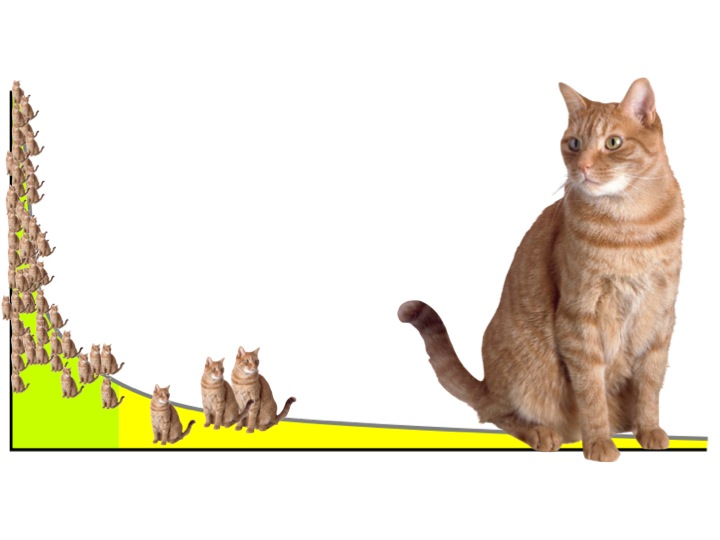
\includegraphics[scale=0.5]{Verchick-cats-graph-2}}} % Image background
\centering
\vspace*{5cm}
\par\normalfont\fontsize{35}{35}\sffamily\selectfont
\textbf{Прикладная стастистика}\\
{\LARGE  ФИВТ ОСЕНЬ 2019}\par % Book title
\vspace*{1cm}
{\Huge Лекционные записи}\par % Author name
\endgroup

%----------------------------------------------------------------------------------------
%	COPYRIGHT PAGE
%----------------------------------------------------------------------------------------

\newpage
~\vfill
\thispagestyle{empty}

%\noindent Copyright \copyright\ 2014 Andrea Hidalgo\\ % Copyright notice

\noindent \textsc{Summer Research Internship, University of Western Ontario}\\

\noindent \textsc{github.com/LaurethTeX/Clustering}\\ % URL

\noindent This research was done under the supervision of Dr. Pauline Barmby with the financial support of the MITACS Globalink Research Internship Award within a total of 12 weeks, from June 16th to September 5th of 2014.\\ % License information

\noindent \textit{Версия 0.0.1 , Октябрь 2019} % Printing/edition date

%----------------------------------------------------------------------------------------
%	TABLE OF CONTENTS
%----------------------------------------------------------------------------------------

\chapterimage{cover_header.jpg} % Table of contents heading image

\pagestyle{empty} % No headers

\tableofcontents % Print the table of contents itself

%\cleardoublepage % Forces the first chapter to start on an odd page so it's on the right

\pagestyle{fancy} % Print headers again

%----------------------------------------------------------------------------------------
%	CHAPTER 1
%----------------------------------------------------------------------------------------

\chapterimage{cover_header.jpg} % Chapter heading image
\chapter{Convex Sets}
\chapter{Точные оценки параметров}
\section{Статистики и оценки}
Пусть $(\mathcal{X}, \mathcal{\beta}_{\mathcal{X}}, \mathcal{P})$ - вероятностное статистическая модель, где: 
\begin{remark}
$\mathcal{X} - $ множество всех возможных котиков,
$\mathcal{\beta}_\mathcal{X} - $  сигма алгебра над котиками,
$\mathcal{P} =  \{P_\theta : \theta \in \Theta\} - $  параметрическое семейство распределений,
$\Theta - $ множество параметров.
\end{remark}
Пусть $(X_1, \cdots, X_n) - $ выборка из неизвестного распределения $P \in \mathcal{P}$
\begin{defi}[Статистика]
Пусть $(E, \mathcal{E}) - $ измеримое пространство. Тогда измеримая функция $S:\mathcal{X} \rightarrow E$  называется статиской. \\
Если $E = \Theta$ то $S(x) - $ оценка $\theta$.
\end{defi}

\begin{exa}
Пусть $X = (X_1, \cdots , X_n) - $ дейсвительная выборка, т.е $\mathcal{X} = \mathrm{R}$ 
\begin{enumerate}
\item Выборочные характеристики: 
\begin{itemize}
\item $ \overline{g(X)}$ $ = \frac{1}{n} \sum_{i=1}^{n} g(X_i)$ - выборочная характеристика функции $g(X) - $ борелевская 
\item $\overline{X} = \frac{1}{n} \sum_{i=1}^n X_i - $  выборочное средние
\item $\overline{X^k} = \frac{1}{n}\sum_{i=1}^n X_i - k $ выборочный момент 
\end{itemize}
\item Функция от выборочных характеристик т.е функции вида $h(\overline{g_1(x)}, \cdots , \overline{g_k(x)})$
\begin{itemize}
\item $g_1(x) = x^2\,, g_2(x) = x\,, h(x,y) = x - y^2$\\ $h(\overline{g_1(x)},\overline{g_2(x)}) = h(\overline{X^2}, \overline{X}) = \overline{X^2} - \overline{X}^2 = S^2 - $ выборочная дисперсия 
\end{itemize}
\item Порядковые статистики 
\begin{itemize}
\item Упорядочим нашу выборку по возрастанию и обозначим её вот так: $$(X_{(1)}, \cdots , X_{(n)})$$ $X_{(k)} - $ $k$ порядковая статистика, $(X_{(1)}, \cdots , X_{(n)}) - $ называется вариационным рядом 
\item \textit{Численный пример.} Пусть у нас есть выборка $(X_1, X_2, X_3) = (2, 5, 1)$\\ $\overline{X} = \frac{2+5+1}{3} = \frac{8}{3}$ \\ $\overline{X^2} = \frac{2^2+ 5^2 + 1^2}{3} = 10$ \\ $S^2 = \overline{X^2} - \overline{X}^2 = 10 - (\frac{8}{3})^2 = \frac{26}{9}$ \\$(X_{(1)}, X_{(2)} , X_{(3)}) = (1,2,5)$
\end{itemize}
\end{enumerate}
\end{exa}
\section{Свойство оценок}
\begin{remark}
Для распределения $P_\theta$ будем обозначать так:
\begin{itemize}
\item $E_\theta - $ математическое ожидание
\item $D_\theta - $ Дисперсия
\item $P_\theta - $ почти наверное 
\item $d_\theta - $ сходимость по распределению
\end{itemize}
\end{remark}
\subsection{Не смещёность оценки }
\begin{defi}
Пусть $X = (X_1 , \cdots , X_2) $ выборка из неизвестного распределения  \\ $P \in \{P_\theta : \theta \in \Theta\}$, $\Theta \in \mathbf{R}^d$. Оценка $\hat{\theta}(x)$ называется не смещённое $\tau(\theta)$ если: $$E\hat{\theta}(X) = \tau(\theta)\text{,  } \forall \theta \in \Theta$$
\end{defi}
\begin{exa}
$\hat{\theta_1}(x) = \overline{X}$ , $\hat{\theta_1}(x) = X_1$ - несмещенные оценки для $\tau(\theta) = E_\theta X_1$
\begin{itemize}
\item $\mathcal{P} = \{\textit{Bern}(\theta) : \theta \in (0,1)\}$ , то $\overline{X}, X_1 - $ несмещенные оценки $\theta$ 
\item $\mathcal{P} = \{\textit{Exp}(\theta) : \theta > 0\}$, то $\overline{X}, X_1 - $  несмещённые оценки $1 / \theta$ 
\end{itemize}
\end{exa}
\subsection{Асимптотические свойства}
Пусть $X = (X_1, X_2,  \cdots) - $ выборка не ограниченного размера из распределения $P \in  \{P_\theta : \theta \in \Theta\} $

\begin{defi}
\label{def_as_property}
\\

\begin{enumerate}
\item Оценка $\hat{\theta}_n(X_1, \cdots, X_n)$ - называется состоятельной оценкой $\theta$ если: $$\hat{\theta}_n(X_1, \cdots, X_n) \xrightarrow[n \rightarrow \infty]{P_\theta} \theta \textbf{,  }\forall \theta \in \Theta $$
\item Оценка $\hat{\theta}_n(X_1, \cdots, X_n)$ называется сильно состоятельной оценкой $\theta$ если $$\hat{\theta}(X_1, \cdots, X_n) \xrightarrow[n \rightarrow \infty] {P_\theta - \textit{п.н}}  \theta ,\s \forall \t \in \T$$
\item Оценка $\H_n \X$ - называется асимптотической нормальной оценкой $\t$, если выполнено такое свойство: $$\sqrt{n}(\H_n \X - \t)  \DT \mathcal{N}(0,\Sigma) ,\s \forall \t \in \T $$ где $\Sigma(\t) - $ асимптотическая матрица ковариации, $\sigma^2(\t)$ - асимптотическая дисперсия.  
\end{enumerate}
\end{defi}
\begin{coro}
\begin{enumerate}
\item Состоятельность - при больших $n$ вероятность отклонения оценки $\HT$ от $\t$, нет численной характеристики степени отклонения 
\item Асимптатической нормальности  - числанная характеристика степени отклонения. \\ Пусть  $\HT - $ а.н.о. $\t$ с асимптатической дисперсией $\sigma^2(\t)$ $$\H \DT \mathcal{N}(\t, \sigma^2(\t) / n)$$ в многомерном случае $\Sigma(\t) - $ задаёт трубу в которой лежит оценка 
\end{enumerate}

\end{coro}

\begin{exa}
Пусть $\X$ - выборка из распределения Лапласа со сдвигом $\t$ плотностью $p_\t(x) = \frac{1}{2} e^{-|x-\t|}$ $,\s E_\t X_1= \t, \s D_\t = 2$\\ УЗБЧ: $\overline{X} \PPT \t \rightarrow - $ сильно состоятельная оценка $\t$  \\ ЦПТ: $\sqrt{n} (\overline{X} - \t) \DT \mathcal{N}(0,2)$ 
\end{exa}

\begin{proposition} Сильная состоятельность $\rightarrow$ Состоятельность, Асимптотическая нормальность $\rightarrow$ Состоятельность
\end{proposition}
\begin{proposition}
Пусть $\X - $ выборка такая что $E_\t |X_1|^{2k} < + \infty$. Тогда $\overline{X_k} - $ не смещенная, (сильно) состоятельная, асимптотическая нормальная оценка $E_\t X_1^k$ 
\end{proposition}

\section{Наследование свойств}
\textbf{Цель}: получить оценку для $\tau(\t)$, обладающие некоторым набором свойств, если имеестя оценка для  $\Psi(\t)$ с тем же свойствами. 

\begin{theorem}[О наследование сходимости]
\label{th_nasledovanoiy_shod}
Пусть $(\xi_n , n\in \mathbb{N})$, $\xi - $ случайный вектор размерности $d$, тогда если :
\begin{enumerate}
\item Если $\xi_n \PT \xi$ и $h: \mathbb{R}^d \rightarrow \mathbb{R}^k$ и $h$ непрерывная тогда $ h(\xi_n) \PT h(\xi)$ 
\item Аналогично для подчинаверной сходимости 
\item Если $\xi_n \d \xi$ и $h: \mathbb{R}^d \rightarrow \mathbb{R}^k - $ непрерывная то $h(\xi_n) \d h(\xi)$
\end{enumerate}
\end{theorem}
\begin{proof}[Доказательство \href{https://youtu.be/EL-V_0kWRoI?t=951}{Live}] 


\end{proof}

\begin{exa}
Пусть  $(\xi_n , n\in \mathbb{N}) - $ независимо одинаково распределённый случайные величины, такие что $E \xi_n = a \neq 0$, $D\xi_n < + \infty$ \\ ЗБЧ: $\frac{S_n}{n} \PT a, $ где $S_n = \xi_1 + \cdots + \xi_n$ \\ Рассмотрим $h(x) = 1/x$ и применим теорему: \\ $h(S_n/n) = \frac{n}{S_n} \PT \frac{1}{a} = h(a)$   
\end{exa}

\begin{proposition}
Пусть $\H -$ (сильно) состоятельная оценка $\t$ пусть $\tau$ непрерывна на $\T$. Тогда $\tau(\H) - $ (сильно) состоятельная оценка $\tau(\t)$ 
\end{proposition}

\begin{lemma}[\href{https://youtu.be/Ys7hMhGSnyE?t=5077} {Лемма Слуцкого}]
\label{lemma_sluc}
Пусть $(\xi_n , n\in \mathbb{N}) , (\eta_n , n\in \mathbb{N})$ $\xi - $ случайные величины, $c \in \mathbb{R}$. Пусть $\xi_n \d \xi$ , $\eta_n \d c$, тогда $\xi_n + \eta_n \d \xi + c$, $\xi_n \eta_n \d \xi c$
\end{lemma}
\begin{theorem}[\href{https://youtu.be/Ys7hMhGSnyE?t=5338}{О производной}]
\label{th_derivative}
Пусть$(\xi_n , n\in \mathbb{N}), \xi -$ случайный вектор размерности $d$ такие что $\xi_n \d \xi$ и $h:\mathbb{R}^d \rightarrow \mathbb{R}^k - $ непрерывна дифференцируема в точки $a \in \mathbb{R}^d$ и последовательность $b_n > 0, b_n \rightarrow 0$. \\ Тогда $\frac{h(a + \xi_nb_n) - h(a)}{b_n} \d \frac{\partial h}{\partial x}|_a \xi,$ где $\frac{\partial h}{ \partial x}|_a  - $ якобиан в точке $a$ 
\end{theorem}
\begin{proof}[$(d = 1):$]
Определим функцию $H(x) = \begin{cases} \frac{h(x+a) - h(a)}{x}, & \mbox{если } x \neq 0 \\ h'(a), & \mbox{если } x = 0\end{cases}$, эта функция непрерывна в точке $a$ давай   те применим лемму Слуцкого (Лемма: \ref{lemma_sluc}): $\xi_n b_n \d \xi 0 \underbrace{\Rightarrow}_{
\includegraphics[scale=0.08]{SDKCG80ysUQ}} \xi_n b_n \p 0 $. \\
Дальше по теореме о наследование сходимости (Теорема: \ref{th_nasledovanoiy_shod}): 
$$H(\xi_n b_n) = \frac{h(\xi_n b_n+a) - h(a)}{\xi_n b_n} \p \d H(0) = h'(a) $$
Ёще раз применим лемму Слуцкого (Лемма: \ref{lemma_sluc}) (для этого мы подчеркнули то что если \textbf{есть сходимость по $\p$ то есть сходимость и по $\d$}, так же $\eta_n = H(\xi b_n), c = h'(a), \xi_n =  \xi_n$)

$$\underbrace{\xi_n H(\xi_n b_n)}_{\frac{h(a+\xi_n b_n) - h(a)}{b_n}} \d h'(a) \xi$$
\end{proof}
\begin{exa}[\href{https://youtu.be/Ys7hMhGSnyE?t=5927}{Live}]
Пусть $(\xi_n , n\in \mathbb{N}) - $ независимо случайно распределённые с.в. т.ч $E\xi_n = a \neq 0,\s D\xi_n = \sigma^2$, сходится ли следующее выражение (где $S = \xi_1 + \cdots + \xi_n$): 
$$\sqrt{n} \left(\frac{n}{S_n} - \frac{1}{a} \right) \d ?$$
\textbf{ Решение: }
Применяем ЦПТ: $$\sqrt{n} \left(\frac{S_n}{n} - a\right ) \d \mathcal{N}(0,\sigma^2)$$
Дальше воспользуемся теоремой о производной (Теорема: \ref{th_derivative}) с такими величинами  $\xi_n = \sqrt{n} \left(\frac{S_n}{n} - a \right ) $, $\xi \sim \mathcal{N}(0,\sigma^2), $ $h(x) = 1/x,\s b_n = 1/\sqrt{n} $: 
$$\frac{h(a  + b_n\xi_n) - h(a)}{b_n} = \sqrt{n} \left[h \left(a + \frac{1}{\sqrt{n}} \sqrt{n} \left(\frac{S_n}{n} - a \right ) \right) - h(a) \right] = \sqrt{n} \left[h \left(\frac{S_n}{n} \right ) - h(a)  \right] \rightarrow$$ $$\rightarrow \sqrt{n} \left[\frac{n}{s_n} - \frac{1}{a}\right] \rightarrow\textit{Теорема(\ref{th_derivative})} \d \xi \left. \left(\frac{1}{x} \right)' \right|_a = -\frac{1}{a^2} \xi \sim \mathcal{N}(0,\sigma^2 / a^4)$$
\end{exa}
\begin{claim}
Если мы расмотрим $\xi_n$ как выборку $\X$ то $1 /\overline{X} - $ это а.н.о. $1/a - $ с а.д. $\sigma^2/a^4$
\end{claim}
\begin{theorem}[\href{https://youtu.be/EL-V_0kWRoI?t=17}{Дельта Метод}] \label{th_delta_method}
Пусть $\H - $ аc. нормальная оценка $\t \in \T \subset \R^d$ с асимптотической матрицей ковариацией $\Sigma(\t)$, и пусть $\tau : \R^d \rightarrow \R^k - $непрерывно дифференцируема функция. \\ Тогда $\tau(\H) - $ ас. нормальная оценка для $\tau(\t)$ с ас. матрицей ковариацией $D(\t)\Sigma(\t)D(\theta)^T, $ где $\D(\t) = \frac{\partial \tau (\t)}{\partial \t}$
\end{theorem}
\begin{proof}
По определению асимптотической нормальной оценки (п. 3. Опр: \ref{def_as_property}). Если  $\H_n -$ ac. нормальная оценка тогда выполняется следующие: $$\sqrt{n}(\H_n - \t) \DT \N (0,\Sigma(\t))$$ Дальше применяем теорему о производной (Теорема: \ref{th_derivative}) с такими параметрами $a = \t, \s h(x) = \tau(x), \s \xi_n = \sqrt{n}(\H_n - \t), \s \xi \sim \N(0, \Sigma(\t)), \s b_n = 1/\sqrt{n} :$
$$\frac{h(a+\xi_nb_n) - h(a)}{b_n} = \frac{h(\t + \frac{1}{\sqrt{n}} \sqrt{n}(\H_n - \t)) - h(\t)}{1/\sqrt{n}} = \sqrt{n} \left[\tau(\H_n) - \tau(\t) \right] \rightarrow$$ $$\rightarrow \textit{Теорема о производной (\ref{th_derivative})} \DT \left. \underbrace{\frac{\partial h(\t)}{\partial \t}}_{D(\t)}\right|_{\t} \xi \sim \N(0, D(\t)\Sigma(\t) D(\t)^T)$$
\end{proof}

\begin{exa}[\href{https://youtu.be/EL-V_0kWRoI?t=504}{Live}] 
Пусть $\X \sim \Exp(\t)$. Тогда из ЦПТ мы зныем: $$\sqrt{n}(\overline{X} - 1/\t) \DT \N(0,1/\t^2) \Rightarrow \overline{X} - \textit{а.н.о. } 1/\t  \textit{ с а.д. } 1/\t^2$$ применяем Дельта Метод (Теорема \ref{th_delta_method}) с функцией $\tau(x) = 1/x:$ $$\tau(\overline{X}) = 1/\overline{X} - \textit{а.н.о. } \tau{(1/\t)} = \t \textit{ с асип. диспе.: } 1/\t^2 \left( \left.\frac{\partial \tau}{\partial x}\right|_{1/\t} \right)^2 = \t^2$$ 

\end{exa}





\end{document}